\documentclass[exb,en]{exercise_5.0}

\deadline{25 .11.2024}

\begin{document}

\section{$SU(3)$ Quark model of the hadrons}
\subsection{}
Let $A\in SU(3)$ and $B\in\mathfrak{su}(3)$. The defining property of $SU(3)$ is that the determinant is one. This reduced the amount of free parameters, from nine in a $3\times3$ matrix to 8. 
$SU(3)$ is thereby an 8-dimensional space, where as $\mathfrak{su}(3)$ must be at least 8-dimensional to be able to generate $SU(3)$.

Starting with the definition of $SU(3)$, one can derive a restraint for matrices of $\mathfrak{su}(3)$:
\begin{align*}
    1&\peq\det A\\
    &= \det (\exp i B )\\
    &= \exp (i \tr B)\\
    \implies \tr B &= 2\pi n \note n\in\Z
\end{align*}
Arbitrarily choosing $n=0$, since it is the simplest, one finds $3\cdot3-1=8$ traceless and linearly independant matrices, which will generate eight linearly independent members of $SU(3)$. Considering that $SU(3)$ is an 8-dimensional space, one can say that they generate $SU(3)$ in its entirety.
Taking a look at $\lambda_1$, one an easily verify, that they indeed span the space of traceless $3\times 3$ matrices, and therefore generate $SU(3)$.

Note: Allowing for $n\neq0$ will introduce more possible linearly independant generators of $SU(3)$, however the space they span does not generate members of $SU(3)$ in general, for example:
\begin{align*}
    A &= \m{2\pi &0&0\\0&0&0\\0&0&0}\note \tr A = 2\pi\\
    e^{iA} &= \I \in SU(3)\\
    e^{i \frac{A}{2\pi}} &= \m{e^{i\pi^2} &0&0\\0&1&0\\0&0&1}\not\in SU(3)
\end{align*}
The eight traceless matrices are the only ones that do span a space of generators, since $\tr(\lambda A) = \lambda \tr A = 0$ for a traceless matrix $A$. Choosing them to be hermitian as well is mathematically not necessary but probably convenient in the context of physics.

\subsection{}
The eigenvectors of $\hat I_3$ are:
\begin{align*}
    \hat I_3 &= \frac12\m{1&0&0\\0&-1&0\\0&0&0}\\
    \ket{ I_3,1/2} &= (1,0,0)\\
    \ket{ I_3,-1/2} &= (0,1,0)\\
    \ket{ I_3,0} &= (0,0,1)
\end{align*}
The eigenvectors of $\hat Y$ are:
\begin{align*}
    \hat Y &= \frac1{3} \m{1&0&0\\0&1&0\\0&0&-2}\\
    \ket{Y,1/3} &= (1,0,0)\\
    \ket{Y,1/3} &= (0,1,0)\\
    \ket{Y,-2/3 } &= (0,0,1)
\end{align*}
$\hat Y$ and $\hat I_3$ evidently share the same three eigenstates.

\subsection{}
For the operator $V_\pm$:
\begin{align*}
    [\hat I_3, \hat V _+] &= \frac12 \hat V_+\\
    [\hat I_3, \hat V _-] &= -\frac12 \hat V_-\\
    \implies [\hat I_3, \hat V_\pm] &= \pm \frac12 \hat V_\pm\\ 
    \\
    \hat I_3 \hat V_\pm \ket{I_3, Y} 
    &= (\hat V_\pm\hat I_3  + [\hat I_3, \hat V_\pm]) \ket{I_3, Y} \\
    &= \hug{\hat V_\pm\hat I_3  \pm \frac12 \hat V_\pm} \ket{I_3, Y} \\
    &= \hat V_\pm\hug{\hat I_3  \pm \frac12 \I} \ket{I_3, Y} \\
    &= \hug{I_3 \pm \frac12}\hat V_\pm \ket{I_3, Y} \\
    \\
    \implies \hat V_\pm\ket{I_3} &\propto \ket{I_3\pm\frac12}
\end{align*}

\begin{align*} 
    [\hat Y, \hat V_+] &= \hat V_+ \\
    [\hat Y, \hat V_-] &= -\hat V_-\\
    \implies [\hat Y, \hat V_\pm] &= \pm \hat V_\pm\\ 
    \\
    \hat Y \hat V_\pm \ket{Y} 
    &= (\hat V_\pm\hat Y  + [\hat Y, \hat V_\pm]) \ket{Y} \\
    &= \hug{\hat V_\pm\hat I_3  \pm \hat V_\pm} \ket{Y} \\
    &= \hat V_\pm\hug{\hat I_3  \pm  \I } \ket{Y} \\
    &= \hug{I_3 \pm 1}\hat V_\pm \ket{ Y} \\
    \implies \hat V_\pm\ket{Y} &= \ket{Y\pm1}\\
    \\
    \implies \Aboxed{\hat V_\pm\ket{I_3,Y} &\propto \ket{I_3\pm\frac12,Y\pm1}}
\end{align*}

For the operator $U_\pm$:
\begin{align*}
    [\hat I_3, \hat U_+] &= -\frac12\hat U_+ \\
    [\hat I_3, \hat U_-] &= \frac12\hat U_-\\
    \implies [\hat I_3, \hat U_\pm] &= \mp \frac12\hat U_\pm\\ 
    \\
    \hat I_3 \hat U_\pm \ket{I_3} 
    &= (\hat U_\pm\hat I_3  + [\hat I_3, \hat U_\pm]) \ket{I_3} \\
    &= \hug{\hat U_\pm\hat I_3  \mp\frac12 \hat U_\pm} \ket{I_3} \\
    &= \hat U_\pm\hug{\hat I_3  \mp  \frac12 \I } \ket{I_3} \\
    &= \hug{I_3 \mp \frac12}\hat U_\pm \ket{ I_3} \\
    \implies \hat U_\pm\ket{I_3} &\propto \ket{I_3\mp\frac12}
\end{align*}

\begin{align*}
    [\hat Y, \hat U_+] &= \hat U_+ \\
    [\hat Y, \hat U_-] &= -\hat U_-\\
    \implies [\hat Y, \hat U_\pm] &= \pm\hat U_\pm\\ 
    \\
    \hat Y \hat U_\pm \ket{Y} 
    &= (\hat U_\pm\hat Y  + [\hat Y, \hat U_\pm]) \ket{Y} \\
    &= \hug{\hat U_\pm\hat Y  \pm \hat U_\pm} \ket{Y} \\
    &= \hat U_\pm\hug{\hat Y  \pm  \I } \ket{Y} \\
    &= \hug{Y \pm 1}\hat U_\pm \ket{ Y} \\
    \\
    \implies \Aboxed{\hat U_\pm\ket{I_3, Y} &\propto \ket{I_3\mp\frac12,Y\pm1}}
\end{align*}

For the operator $I_\pm$:
\begin{align*}
    [\hat I_3, \hat I_+] &= \hat I_+ \\
    [\hat I_3, \hat I_-] &= -\hat I_-\\
    \implies [\hat I_3, \hat I_\pm] &= \pm \hat I_\pm\\ 
    \\
    \hat I_3 \hat I_\pm \ket{I_3} 
    &= (\hat I_\pm\hat I_3  + [\hat I_3, \hat I_\pm]) \ket{I_3} \\
    &= \hug{\hat I_\pm\hat I_3  \pm \hat I_\pm} \ket{I_3} \\
    &= \hat I_\pm\hug{\hat I_3  \pm\I } \ket{I_3} \\
    &= \hug{I_3 \pm 1}\hat I_\pm \ket{ I_3} \\
    \implies \hat I_\pm\ket{I_3} &\propto \ket{I_3\pm1}
\end{align*}

\begin{align*}
    [\hat Y, \hat I_+] &= 0\\
    [\hat Y, \hat I_-] &= 0\\
    \implies [\hat Y, \hat I_\pm] &= 0\\ 
    \\
    \hat Y \hat I_\pm \ket{Y} 
    &= (\hat I_\pm\hat Y  + [\hat Y, \hat I_\pm]) \ket{Y} \\
    &= \hat I_\pm\hat Y \ket{Y} \\
    &= Y \hat I_\pm \ket{Y} \\
    \\
    \implies \Aboxed{\hat I_\pm\ket{I_3, Y} &\propto \ket{I_3\pm1,Y}}
\end{align*}

\subsection{}
Isospin and hypercharge of the three basisvectors where shown to be (task (b)): 
\begin{align*}
    \hat I_3 \ket u &= \frac12\ket u\\
    \hat I_3 \ket d &= -\frac12\ket d\\
    \hat I_3 \ket s &= 0 \ket s \\
\\
    \hat Y \ket u &= \frac13\ket u\\
    \hat Y \ket d &= \frac13\ket d\\
    \hat Y \ket s &= -\frac23 \ket s
\end{align*}

Now for the strangeness $S$:
\begin{align*}
    Y &= B+S\\
    S &= Y-B = Y - \frac13\\
    \implies \hat S &= \hat Y - \frac13\I\\
    \\
    \hat S \ket u &= 0\ket u\\
    \hat S \ket d &= 0\ket d\\
    \hat S \ket s &= -1 \ket s \\
\end{align*}

\subsection{}
\begin{figure}[H]
    \centering
    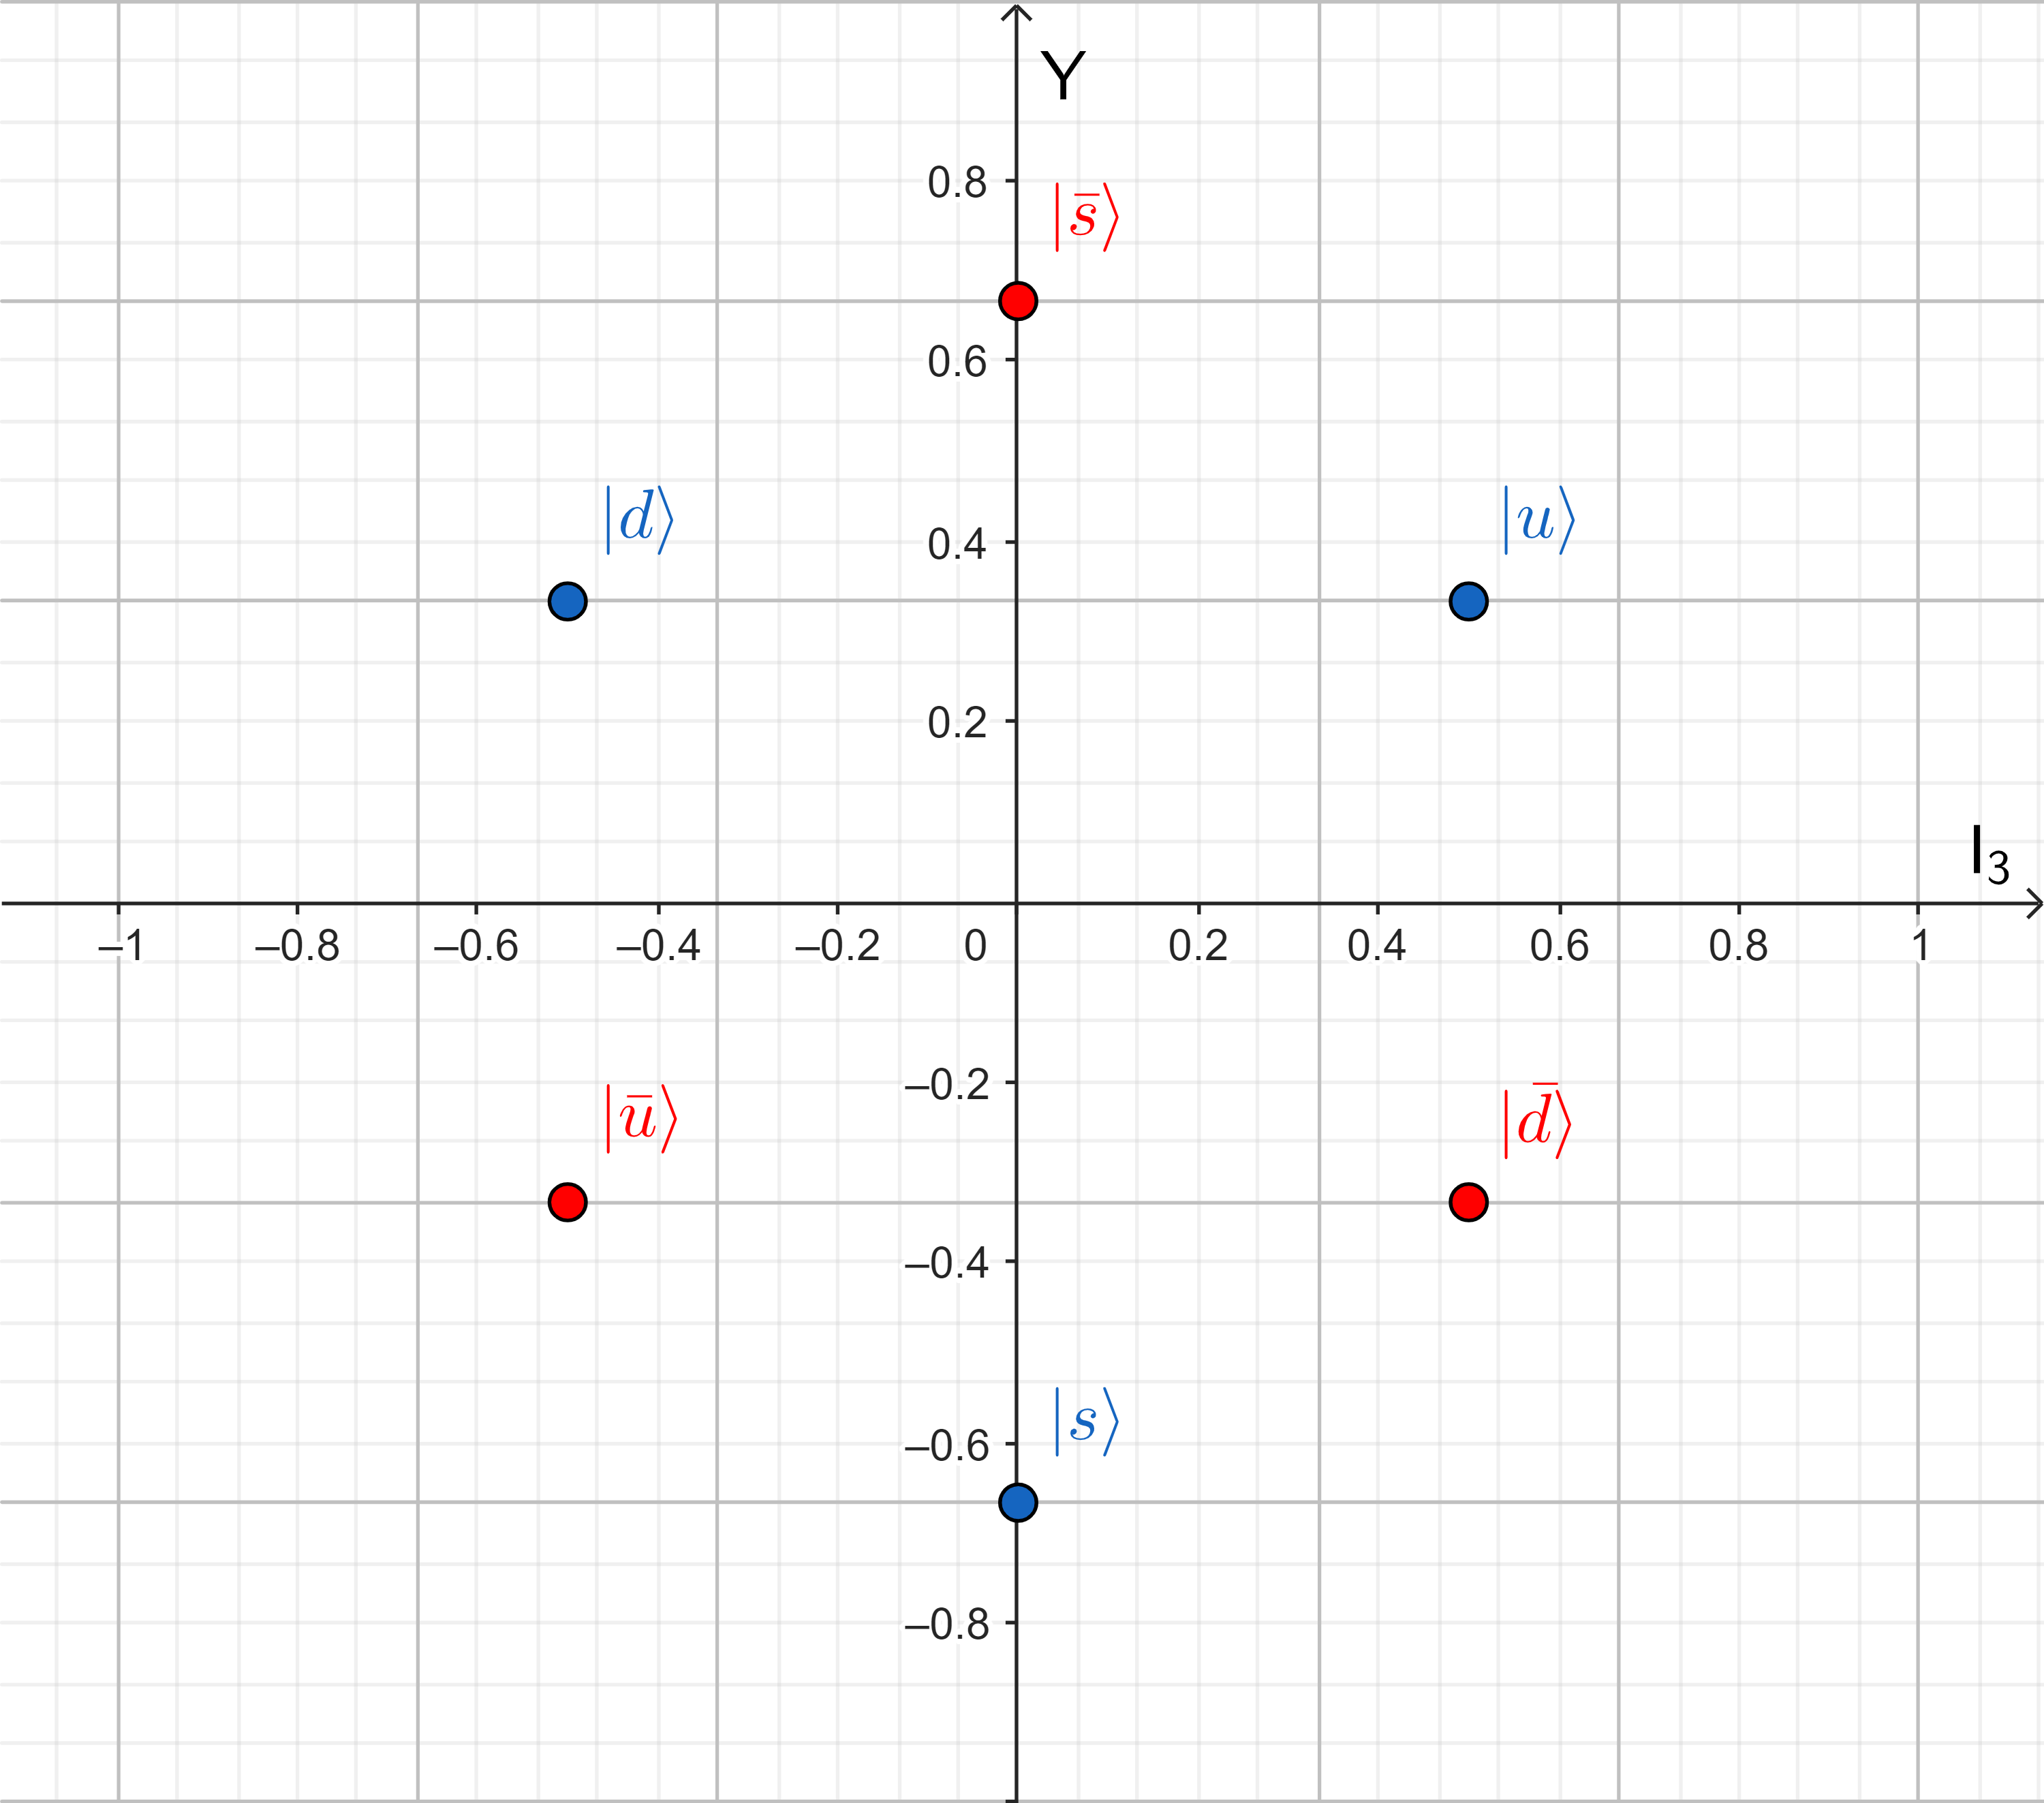
\includegraphics[width=.8\textwidth]{geogebra.png}
\end{figure}

\subsection{}
\inputpy[lastline=56]{}{4.py}
\begin{figure}[H]
    \centering
    \includesvg[width=1\textwidth]{effects_of_shiftoperators.svg}
    \caption{In the graphic, the triplet from the previous task is displayed, along with all states affected by the shift operators. Most states get mapped to (0,0,0) and are therefore omitted. Additionally, states that are mapped to the same point have been slightly separated for better clarity.}
\end{figure}


\subsection{}
\subsubsection{}
Using the graphics on the problem sheet, it is obvious that 
$[3]\otimes[\bar 3]$ decomposes to $[1]\oplus [8]$. 

\subsubsection{}
To decompose $[3]\otimes [3]\otimes[3]$, it is easiest to decompose $[3]\otimes[3]$ first. Again taking a look at the graphical decomposition $[3]\otimes[3]$ decomposes to $[\bar 3]\oplus[6]$. 
\begin{align*}
    [3]\otimes[3]\otimes[3] 
    &= [3]\otimes([\bar 3]\oplus[6])\\
    &= [3]\otimes[\bar 3]\oplus[3]\otimes[6]\\
    &= [1]\oplus[8]\oplus[3]\otimes[6]\\
\end{align*}
The remaining decomposition is $[3]\otimes[6]$ and it decomposes to $[10]\oplus[8]$. The composition of $[3]\otimes [3]\otimes[3]$ therefore is:
\begin{align*}
    [3]\otimes[3]\otimes[3] 
    &= [1]\oplus[8]\oplus[3]\otimes[6]\\
    &= [1]\oplus[8]\oplus[8]\oplus[10]
\end{align*}

\subsection{}

\inputpy[firstline=60]{}{4.py}

\begin{figure}[H]
    \centering
    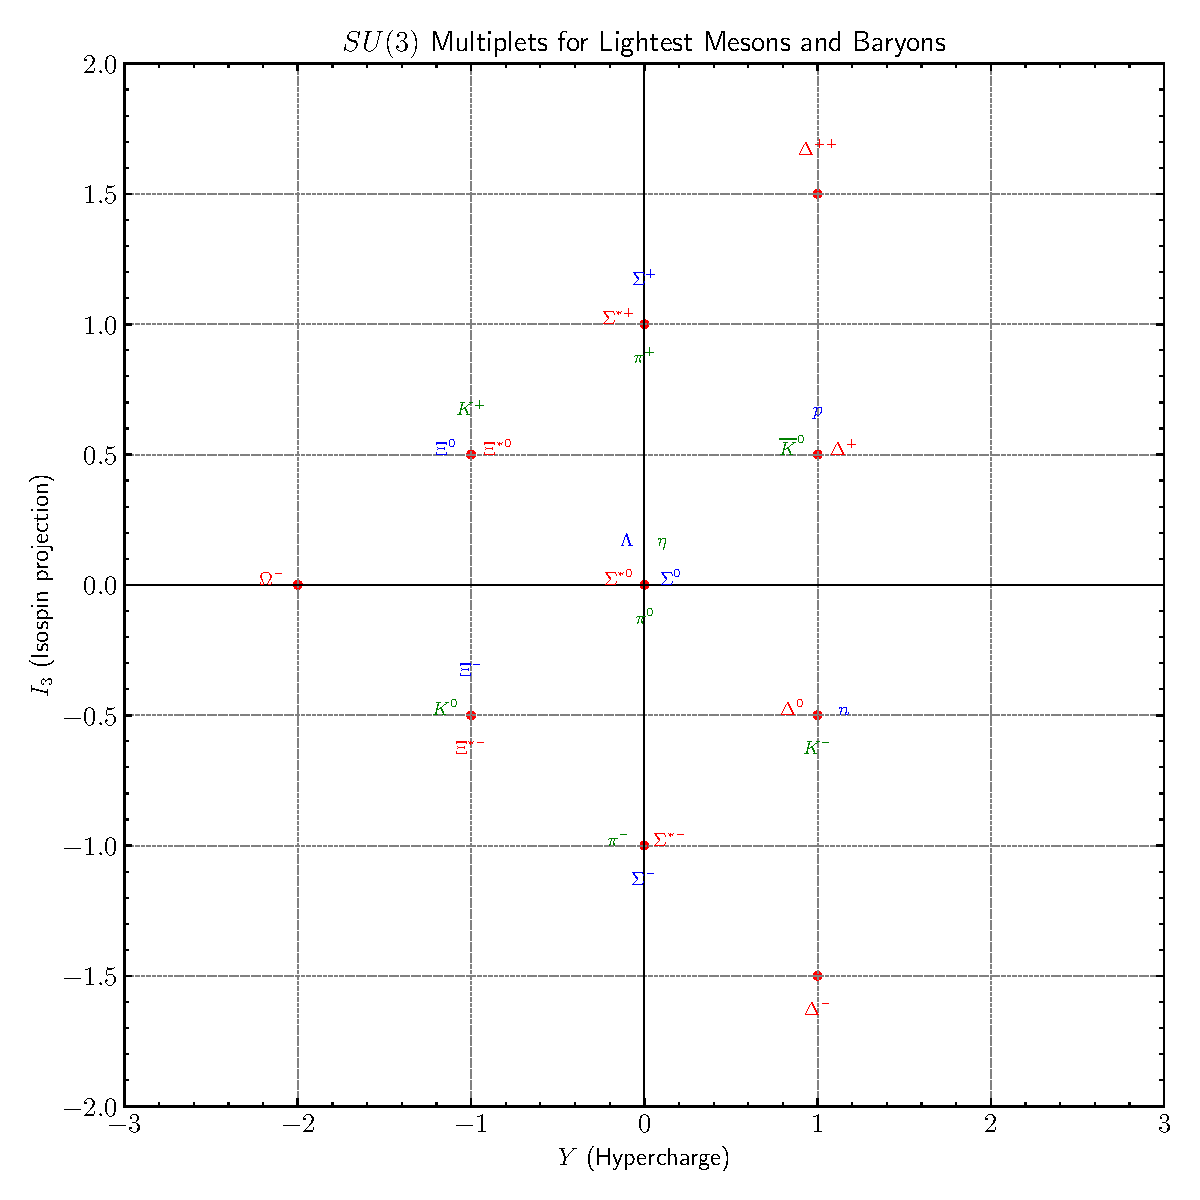
\includegraphics[width=1.0\textwidth]{tmp.pdf}
    \caption{What a tedious task... Mesons, including the pions, kaons, and the $\eta$ meson, are shown in green, while baryons from the $SU(3)$ octet, such as protons, neutrons, and $\Lambda$ baryons, are represented in blue. Baryons from the $SU(3)$ decuplet, including the $\Delta$, $\Sigma^P$, $\Xi^*$ resonances, and the $\Omega^-$ baryon, are displayed in red.}
\end{figure}

\subsection{}
The breaking of the $SU(3)$ symmetrie is caused by the fact that the different quarks dont have the same mass and interact differently under the weak interaction. The symmetrie would be exact if only the strong force is  looked at.

\subsection{}
The relevant particles, their constituents and their masses are:
\begin{itemize}
    \item {Proton/Neutron (\(N\))}: \(uud\) or \(udd\implies m_N=3 m_u + W_B\)
    \item {Xi (\(\Xi\))}: \(uss\) or \(dss\implies m_\Xi=m_u + 2m_s + W_B\)
    \item {Lambda (\(\Lambda\))}: \(uds\implies m_\Lambda= 2m_u + m_s+ W_B\)
    \item {Sigma (\(\Sigma\))}: \(uus\), \(uds\), or \(dds\implies m_\Sigma=2 m_u + m_s + W_B\)
\end{itemize}

Using this the mass relation can be shown:
\begin{align*}
    \frac{m_N + m_\Xi}{2} &= \frac{3m_\Lambda + m_\Sigma}{4}\\
    \frac{(3 m_u + W_B) + (m_u + 2m_s + W_B)}{2} &= \frac{3(2m_u + m_s+ W_B) + (2 m_u + m_s + W_B)}{4}\\    
    2m_u + m_s + W_B &= 2m_u + m_s+ W_B
\end{align*}

The experimental masses are approximatly:
\begin{align*}
    m_N \approx 938 \u{MeV}\\
    m_\Xi \approx 1315 \u{MeV}\\
    m_\Lambda \approx 1115 \u{MeV}\\
    m_\Sigma \approx 1192 \u{MeV}
\end{align*}

Plugging these values into the mass relation yields:
\begin{align*}
    \frac{938 + 1315}{2} &= \frac{3\cdot 1115+ 1192}{4}\\
    1126.5 &= 1134.25
\end{align*}
The relation holds quite well, with a small discrepancy, which can be attributed to the simplified assumptions made.


\end{document}